For applications in which the input-output mapping is static, Feed-Forward Neural Networks suffice most of the time.
As soon as temporal correlations between the samples exists, this static assumption becomes inadequate \citep{tsoi1997recurrent}. 
Temporal correlation can mean that the input instances happened sequentially or that an order persists between them. 
Feed-Forward Neural Networks do not incorporate these structural properties of the input which may hold valuable information for task in which the sequential nature of data is of relevance.

Therefore the concept of Recurrent Neural Networks (RNN) is introduced for sequences of inputs and the ability to capture statistical regularities in them \citep{goldberg2017neural}.

These regularities are captured by the fact that previous inputs may influence the current information flow by a recurrent state element specific to RNNs. 
So the flow of information is not only forward, but has a cyclic element to it \citep{jurafsky2021}. 
Incorporating such feedback loops allows the neural network to exhibit a temporal dynamic behaviour and, as \citet{embedding2020pilehvar} puts it, remember the past. 
In figure \ref{fig:RNN_1} this is exemplified by the connection of the same unit in the model with itself at the time the next input instance is fed through it.

\begin{figure}
  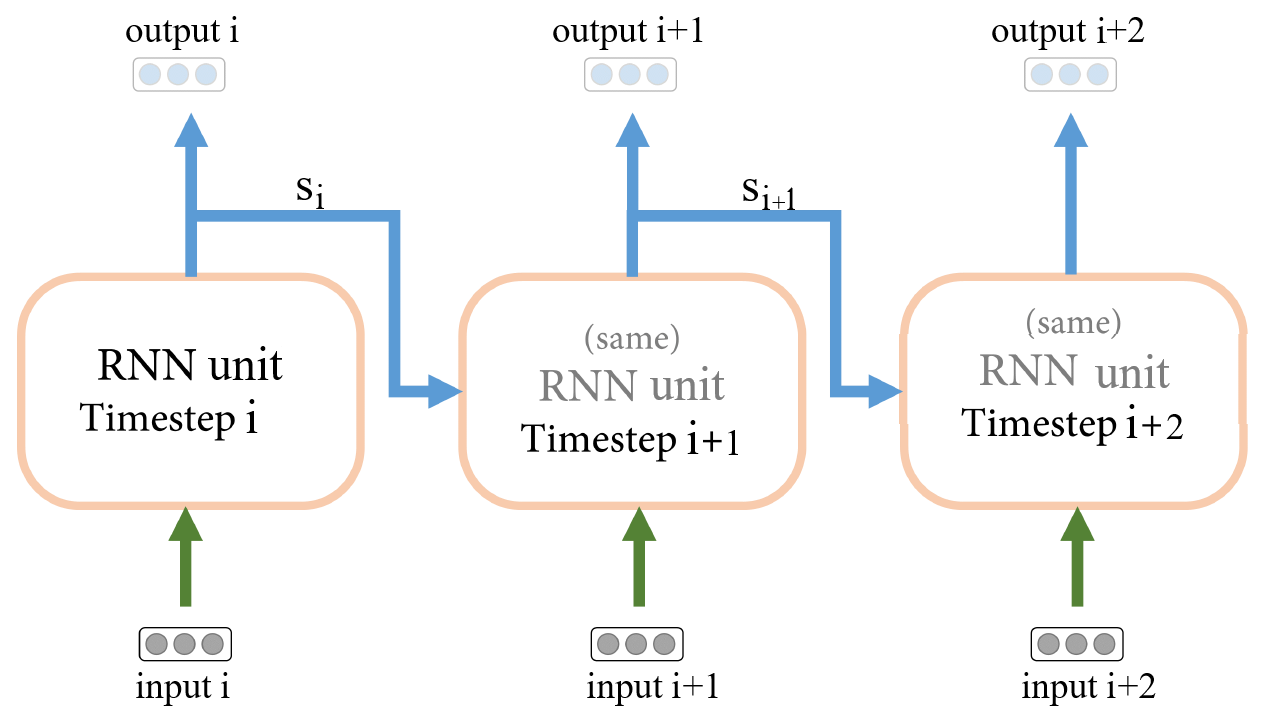
\includegraphics[width=\linewidth]{Pictures/Pilehvar_20_RNN.png}
  \caption{Adapted and modified from \citet{embedding2020pilehvar}: Visualization of a single unit of a RNN for sequential data. These three time correlated or sequential instances $i, i+1, i+2$ show the recurrence of the model by the two arrows between the unit in different time steps.}
  \label{fig:RNN_1}
\end{figure}


On a mathematical level this is achieved by making a prediction at point $i$ in a sequence dependent on all inputs up to index $i$ in the sequence, $x_{1:i-1}$. 
In general terms this can be represented, without specifying a concrete model architecture, by a recursive state element $s$. 
It incorporates the information of previous time steps and is combined with the current input to generate the recursive state element for the current prediction and for providing memory for the next time step.

\begin{equation}
\label{eq:R}
    s_i = R(s_{i-1}, x_i)
\end{equation}

In equation \ref{eq:R} the letter 'R' is used as a placeholder for a multitude of recursive techniques for which the model architectures may incorporate the information of former states. In case of the first input vector the previous recursive state element $s$ is a zero vector.
A concrete implementation of $s$ will be given in more detail for the architecture of LSTM Neural Networks in \ref{nn_lstm}.

One major difficulty when training Neural Network occurs due to the so called vanishing gradient problem. 
As explained in \ref{nn_train} the adjustment of weights and biases of the model happens according to the calculated gradients and derivatives starting at the loss and propagating backwards.
Since the calculation of gradients uses the results of the preceding steps in the backwards pass through the broken down equations of the whole model, 
the values of the gradients may vanish or, in cases of activation functions not presented here, explode when put through the activation functions used on the layers \citep{embedding2020pilehvar}.

If one considers the gradients of activation functions presented in figure \ref{fig:AF} one can assess that their gradients are in the range of values between 0 to 1. 
As their gradients become close to 0 and the backpropagation multiplies these low values several times, the resulting gradients may get vanishingly low \citep{tsoi1997recurrent}.

This problem especially arises for Recurrent Neural Networks since it incorporates a recursive element in the model to capture the structural properties of the input data.
Therefore an increasing number of multiplications with very low values may take place once the error backpropagation has passed through some recurrences. 
Consequently the adjustments of the according parameters happens only at a vanishingly low rate that makes the training procedure very inefficient. 
The problem of inefficiently capturing long-range dependencies was thoroughly investigated by \citet{gradient1994bengio}.

Another difficulty these models deal with is the fact that the recurrent state element \textbf{s} has to provide relevant information for the current decision while at the same time try to retain information for future decisions. 

One way to deal with these problems is to use gated varients of Recurrent Neural Networks.


